\section{Background and Threat Model}
In this section, we first present an introduction to software-based 
side-channel attacks. Moreover, we analyze the root cause of many
software-based side-channels. We find many of them are caused by
two specific side-channel vulnerabilities, secret-dependent control-flow transfers and
secret-dependent memory accesses. Therefore, we will focus on identifying
and quantifying those leakages in the paper. After that, we 
discuss existing methods on side-channel detection and quantification.

\subsection{Software-based Side-channels}
Side-channels are information channels that can leak sensitive information 
unconsciously through different execution behaviors.  Fundamentally, those 
differences were caused by shared hardware
components (e.g., the CPU cache, the TLB and DRAM) in modern computer systems.
Depending on the layer causing side-channels, we can classify them 
into the following types of side-channel attacks.

For example, cached-based side-channels rely on the time differences 
between cache miss and cache hit. We introduce two common attack strategies,
namely Prime+Probe and Flush+Reload.
Prime+Probe targets a single cache set. The attacker preloads cache set with
its own data and wait until the victim execute the program.
If the victim accesses the cache set and evicts part of 
the data, the attacker will experience a slow measurement. If not, 
it will be fast. By knowing which cache set the target
program accesses, the attacker can infer locations of
the sensitive information. Flush+Reload targets a single cache line. 
It requires the attacker and the victim share the same memory address space.
During the ``flush'' stage, an attacker 
flushes the ``monitored memory'' from the cache. Then the attacker
waits for the victim to access the memory. In the next phase, the 
attacker reload the ``monitored memory''. By measuring the time difference, the
attacker can infer the sensitive information.

There are some other types of side-channels which target different hardware layers other than  
CPU cache as well.
For example, the controlled-channel attack~\cite{7163052},
where an attacker works in the kernel space, can infer sensitive data in the shielding systems by
observing the page fault sequences after restricting some code and
data pages. 

\begin{figure}[]

\noindent\begin{minipage}{0.45\linewidth}
    \noindent
\begin{lstlisting}[numbers = none]
unsigned long long r;
int secret[32];
while(i>0){
    r = (r * r) % n;
    if(secret[--i] == 1){
        r = (r * x) % n;
    }
}
\end{lstlisting}
\caption{Secret-dependent control-flow transfers}
\end{minipage}
\hfill
\begin{minipage}{0.45\linewidth}
\begin{lstlisting}[numbers = none]
static char Fsb[256] = {...}
... 
uint32_t a = *RK++ ^ \ 
(FSb[(secret)) ^
(FSb[(secret >> 8)] <<  8 ) ^
(FSb[(secret >>16)] << 16 ) ^
(FSb[(secret >>24)] << 24 );
...
\end{lstlisting}
\caption{Secret-dependent memory accesses}
\end{minipage}
\end{figure}

The key intuition is that each side-channels above happens when the program accesses different 
memory addresses if the program has different sensitive inputs. More specifically, if 
a program show different patterns in control transfers or data accesses when the program 
processes different sensitive inputs, the program could possibly have side channels vulnerabilities. 
Different kinds of side-channels can be exploited to retrieve information
in various granularities. For example, many cache channels can observe cache accesses
at the level of a cache line. For most CPU, one cache line holds 64 bytes of data. So
the low 6 bits the address is irrelevant in causing those cached-based side-channels. 

%\lstinputlisting[language=c, 
%                 numbers=left,
%                 caption={Sample code shows secret-dependent memory access and 
%                          secret-dependent control-flow transfer.},
%                 captionpos=b,
%                 label={code:background},
%                 frame=single,
%                 basicstyle=\fontsize{7}{9}\selectfont\ttfamily]
%                 {sample_code/background.c}

%For example, the above code~\ref{code:background} show a simple encryption function that
%has the two kinds of side-channels. At line 11, depending on the value of a key,
%the code will access the different entry in the predefined table. At the
%line 13, the code will do a series of computation and determine if the code in the if
%branch is executed or not. Such vulnerabilities are called the memory-based 
%side-channles. We identify and quantify the leakage of the two kinds of vulnerabilities 
%in the paper.

\subsection{Information Leakage Quantification}
 
Given an event $e$ that occurs with the probability $p(e)$, if the event $e$ happens, 
then we receive
\begin{displaymath}
    I = - \log_2p(e)
\end{displaymath}
bits of information by knowing the event $e$.
Considering a char variable $a$ with one byte storage size in a C program, its value 
ranges from 0 to 255.  Assume
 \textit{a} has the uniform distribution. If at one time we observe that $a$
equals $1$, the probability of this observation is $\frac{1}{256}$. So the information we get is 
$-\log(\frac{1}{256}) = 8$ bits, which is exactly the size of the char variable in the C program.

Existing works on information leakage quantification uses Shannon entropy,  
min-entropy \cite{10.1007/978-3-642-00596-1_21}, and max-entropy.
In these frameworks, the input sensitive
information $K$ is viewed as a random variable. 

Let $k_i$ be one of the possible
value of $K$. The Shannon entropy $H(K)$ is defined as
\begin{displaymath}
    H(K) = - \sum_{k_i {\in} K}p(k_i)\log_2(k_i)
\end{displaymath}

Shannon entropy can be used to quantify the initial uncertainty about the sensitive
information. It measures how much information is in a system.

Min-entropy describes in the information leaks from the most likely outcome.
For example, min-entropy can be used to describe the best chance of success in guessing 
one's password in one chance, which is defined as 
\begin{displaymath}
    \mathit{min\text{-}entropy} = - \log_2(p_{max})
\end{displaymath}

Max-entropy is defined solely on the number of possible observations. 
  %It is equal to $-\log_2{n}$.
\begin{displaymath}
    \mathit{max\text{-}entropy} = -\log_2{n}
\end{displaymath}
As it is easy to compute, most recent works use 
max-entropy as the definition of the amount of leaked information.

To illustrate how above definitions work, we consider the following
code fragment. 

\begin{lstlisting}[xleftmargin=.03\textwidth,xrightmargin=.01\textwidth]
uint_8 key[2];
get_key(key);              // 0 <= key[0], key[1] < 256
if (key[0] + key[1] < 8) {
    A();                   // branch 1
}
if (key[0] > key[1]) {     // branch 2
    B();
}
\end{lstlisting}

Suppose an attacker can observe if branch 1 and branch 2 are executed or not, 
an attacker can have four different observations:
$\emptyset$ for neither branch 1 nor branch 2 executed,
$\{1\}$ for only branch 1 executed,
$\{2\}$ for only branch 2 executed, and
 $\{1, 2\}$ for both branch 1 and branch 2 executed.
If $key$ has uniform distribution, we can calculate the corresponding
possibility by counting the number of possible solutions.
\begin{table}[ht]
    \centering

 %  \resizebox{.8\columnwidth}{!}{

\begin{tabular}{l|cccc}
    \hline
%Observation (o)     & $\emptyset$ & ${\{1\}}$ & ${\{2\}}$ & ${\{1, 2\}}$ \\ \hline
%Number of Solutions &  32876 & 20 & 32634 & 16 \\ \hline
%Possibility (p)     & 0.5016 & 0.0003 & 0.4980  & 0.0002   \\
Observation ($o$)  & $\emptyset$ & ${\{1\}}$ & ${\{2\}}$ & ${\{1, 2\}}$ \\ \hline
Number of Solutions &  32876 & 20 & 32634 & 16 \\ \hline
Possibility (p)     & 0.5016 & 0.0003 & 0.4980  & 0.0002   \\
    \hline
\end{tabular}
%    }
\end{table}
According to the definition, min-entropy equals to 
\begin{displaymath}
    \mathit{min\text{-}entropy} = -\log_2{0.5016} = 1.0\ \mathit{bits}
\end{displaymath}
Because the above code has four different observations, max-entropy equals to 
\begin{displaymath}
    \mathit{max\text{-}entropy} = -\log_2{4} = 2.0\ \mathit{bits}
\end{displaymath}
Shannon entropy, according to the definition, equals to 
\begin{displaymath}
    \mathit{Shannon\text{-}entropy} = 1.0\ \mathit{bits}
\end{displaymath}





------\fixme{CLEANUP - begin}------

Note, if i understand correctly, you'll have the following:
\begin{enumerate}
\item Shannon entropy
\item min-entropy
\item max-entropy
  \item mutual information
\end{enumerate}
clean up the following material and introduce mutual information.
After that, we'll instruct you on how to add some additional information
that can help our paper.

Now we provide a concrete example to show how the two types of quantification definition works and show that
how our method is different.

\vspace{3pt}
\textbf{Maximal Leakage.} 
Depending on the value of key, the code can run four different branches which corrosponding to 
four different observations. Therefore, by the maximal leakage definition, the leakage equals to 
$\log4 = 2$ bits.

\vspace{3pt}
\textbf{Mutual Information.}
If the key satisfies the uniform distribution, the probability of the code runs each branch
can be computed with the following result.  

\begin{table}[h]
\centering
%\resizebox{\columnwidth}{!}{
\begin{tabular}{|c|c|c|c|c|}
\hline
Branch & A     & B      & C      & D       \\ \hline
Possibility      & 1/256 & 64/256 & 64/256 & 127/256 \\ \hline
\end{tabular}
%}
\caption{The distribution of observations}
\end{table}

Therefore, the leakage equals to 
$\frac{1}{256}\log\frac{1}{256} + \frac{1}{4}\log\frac{1}{4}*2 + \frac{127}{256}\log\frac{127}{256} = 1.7$ bits.


------\fixme{CLEAN UP - continue}------

\section{\tool{} Leakage Definition}
\label{trace_qif}
In the section, we discuss how \tool{} quantifies the amount of
leaked information. \tool{} is a dynamic-based approach to 
quantifying the leaked information. We will first present 
the limitation of existing quantification metrics. After
that, we introduce the abstract of the model and math notations 
for the paper and propose our method.

\subsection{Problem Setting}
Existing static-based side-channel quantification works~\cite{182946,Wichelmann:2018:MFF:3274694.3274741 } define information leakage
using max entropy or Shannon entropy. These definitions provide a strong security guarantee
when trying to prove a program is secure enough if zero bit of information is leaked 
reported by their approaches. However, it is useless if the tool report the program leaks
some information. Moreover, those metrics does not apply to static method.


\begin{figure}[h!]
    \centering
\begin{lstlisting}[xleftmargin=.03\textwidth,xrightmargin=.01\textwidth]
uint8_t password = input();
if(password == 0x1b){
    pass();     //branch 1
}else{
    fail();     //branch 2
}
\end{lstlisting}
\caption{A dummy password checker}
\label{figure:password checker}
\end{figure}

We consider the above dummy password checker in ~\ref{figure:password checker}.
The program will take a 8 bit number as the input and check if the input is the
correct password. 
If an attacker knows the
code executes branch $\{{1\}}$ by side-channel attacks, he can infer the password equals to 0x1b,
in which case the attacker can fully retrieve the password.
Therefore, the total information leakage should be 8 bits, which equals to the size
of the sensitive input if an attacker observes the code executes branch $1$ . 

However, previous static-based approach can not precisely reflect the sensitivity of the leakage.
According to the definition of Shannon entropy, the leakage will be $\frac{1}{256}*\log_{2}\frac{1}{256} + 
\frac{255}{256} *\log_{2}\frac{255}{256}= 0.24$ bits. Because the program has two branches, tools
based on max-entropy will report the code has $\log_2{2} = 1$ bit leakage.

Both approaches fail to tell how 
much information is leaked during the execution precisely.
The problem with existing methods is that they are static-based and the 
input values are neglected by the previous definition. 
They assume the attacker runs the program multiple times with many different sensitive 
information as the input. Both Shannon entropy and max entropy give an ``average" 
estimate of the information leakage. However, it is not the typical scenario for an adversary to 
launch a side-channel attack. When a side-channel attack happens, the adversary wants 
to retrieve the sensitive information, in which case the sensitive information is fixed (e.g., AES keys). 
The adversary will run the attack over and over again and guess the value bit by bit. Like the 
previous example, the existing static method does not work well in those situations.
We want to have a theory for dynamic analysis that if the theory says 
an attack leaks $x$ bits of secret information from side-channel vulnerabilities,
then $x$ should be useful in estimating the sensitive level of side-channels.
However, the above method all fails in the real attack model.
\begin{figure}
  \centering
   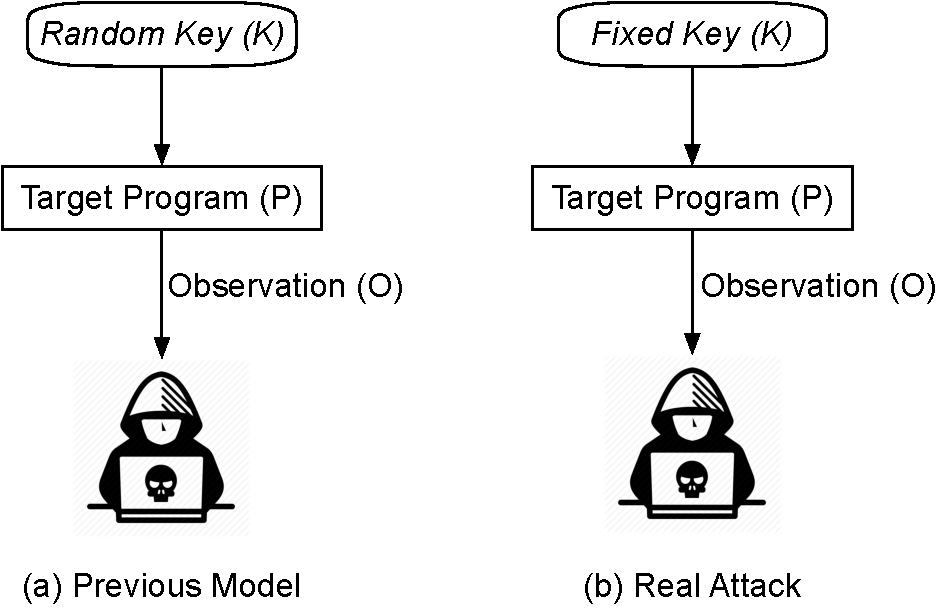
\includegraphics[width=.8\columnwidth]{./figures/RA.pdf}
   \caption{The gap between the real attack and previous model}
\end{figure}


\subsection{Notations}
In the section, we give the necessary definitions and notations for dealing 
with programs and side-channels. We use capital letters (e.g., $A$) to represent 
the set. $|S|$ represents the size of set $A$. We use corresponding small letters
to represents one element in the set (e.g., $a \in A$).

We assume the program ($\beta$) has $K$ as the sensitive input. 
$K$ should be a finite set of keys. The program also takes known messages $M$ as the input. 
The model applies to most of the cryptosystems. For example,
during the AES encryption, $\beta$ is the encryption function. $K$ is AES key and
$M$ is the message to be encrypted. During the execution, an adversary may have some observations ($O$) from the program. Examples of those observations
include timing, CPU usages, and Electromagnetic signals (EM). For this paper, we
consider the secret-dependent control-flows and secret-dependent memory accesses
as the observations.

With the above definitions, we have the following mapping between $\beta$, $K$, $M$, and $O$:

\begin{displaymath}
    \beta(K, M) \rightarrow O
\end{displaymath}

An adversary does not have access to $K$, but he knows $\beta$, $M$, and $O$. 
For one execution of a deterministic program, once $k \in K$ and $m \in M$ are fixed, the 
observation ($o \in O$) is also determined. As an attacker, he knows $\beta$, $o$, 
and $m$. The attacker wants to infer the value of $k$. We use $K^o$ to denote the set of
possible $k$ values that still produce the same observations:

\begin{displaymath}
    K^o = \{ k \in K \, |\, \beta(k, m) \rightarrow o\}
\end{displaymath}
Then the problem of quantifying the amount of leaked information can be transferred into the
following question. 
\emph{How much uncertainty of $K$ can be reduced if an attacker knows $\beta$, $m$, and $o$?}
 
\subsection{Theoretical Analysis}
Now we present our metric to quantify the amount of leaked 
information from dynamic analysis.

In information theory, the mutual information (MI) of is a measure of the mutual dependence 
between the two variables. Here we use MI to describe the leakage between $K$ and $O$, 
which is defined as:

\begin{equation} \label{eq:1}
    I(K;O) = \sum_{k {\in} K}{\sum_{o {\in} O}{p(k, o)\log_2\frac{p(k, o)}{p(k)p(o)}}}
\end{equation}

where $P(k_i, o_i)$ is the joint discrete distribution of $K$ and $O$.
Alternatively, the mutual information can also be equivalently expressed as:
\begin{equation} \label{eq:2}
    I(K;O) = H(K) - H(K|O)
\end{equation}

$H(K|O)$ is the entropy of $K$ conditioned on $O$. It quantifies the uncertainty of $K$
given the value of $O$. In other word, the conditional entropy $H(K|O)$ marks the 
uncertainty about $K$ after the adversary has gained some observations ($O$). 
\begin{equation}
    H(K|O) = - \sum_{o {\in} O} {p(o) \sum_{k {\in} K}{p(k|o)\log_2p(k|o)}}
\end{equation}

In the project, we hope to give a very precise definition of information leakages. 
Suppose an attacker run the target program multiple times with one fixed input, we
want to know how much information he can infer by observing the memory access patterns ($o$).
We come to the simple slogan ~\cite{10.1007/978-3-642-00596-1_21} %% where the information
%% leakage equals:
%% \textbf{Initial uncertainty - remaining uncertainty}
that
\begin{align*}
 & \mathit{Information\ leakage} = \\
 & ~~~~~~ \mathit{Initial\ uncertainty} - \mathit{Remaining\ uncertainty}. 
\end{align*}

Now we come compare the equation~\ref{eq:2} with the above slogan, we will
find $H(K)$ is the $\mathit{Initial\ uncertainty}$ and $H(K|O)$ is
$\mathit{Remaining\ uncertainty}$. During a side-channel attack, 
the observation ($o$) is known.  We have $H(K|O) = H(K|o)$.

Therefore, we define the amount of leaked information as 
\begin{displaymath}
    Leakage = H(K;o) = H(K) - H(K|o)
\end{displaymath}

For a program ($\beta$) without knowing any domain information, any sensitive
input should appear equally. Therefore, for any $k \in K$, $p(k) = \frac{1}{|K|}$.
So we have 
$$H(K) = \sum_{k {\in} K}\frac{1}{|K|}\log_2{|K|} = \log_2{|K|}$$
For any $k' \in K - K^o$, $p(k'|o) = 0$. We can get the following equation:
\begin{align*}
H(K;o) &= - \sum_{k {\in} K^o}{p(k|o)\log_2p(k|o)} 
          - \sum_{k` {\in} (K - K^o)}{p(k'|o)\log_2p(k'|o)}\\
       &= \sum_{k {\in} K^o}\frac{1}{|K^o|}\log_2{|K^o|}\\
       &= \log_2{|K^o|}
\end{align*}

\newtheorem{mydef}{Definition}

\begin{mydef}
\label{def}
Given a program $\beta$ with the input set $K$, 
an adversary has the observation $o$ when the input $k{\in}K^o$. 
We denote it as
$$\beta(K^o, m) \rightarrow	o$$

The leakage $L_{\beta(k)\rightarrow o}$ based on the observation ($o$) is
    $$L_{\beta(k)\rightarrow o} = \log_2{|K|} - \log_2{|K^o|}$$
\end{mydef}

With the new definition, if the attacker observes that the code~\ref{figure:password checker} runs the branch 1, 
then the $K^{o^{1}} = \{\mathrm{0x1b}\}$. Therefore, the information leakage $L_{P(k)=o^{1}} = \log_2{256} - \log_2{1} = 8$
bits, which means the key is totally leaked. If the attacker observes the code runs branch2, the leaked information is 
$L_{P(k)=o^{2}} = \log_2{256} - \log_2{255} = 0$ bit.


We can also calculate the leaked information
from the sample code~\ref{background::side-channel}. As the size of input 
sensitive information is usually public. The problem of quantifying the
leaked information has been transferred into the problem of estimating
the size of input key $|K^o|$ under the condition $o \in O$.

\begin{table}[ht]
    \centering

 %  \resizebox{.8\columnwidth}{!}{

\begin{tabular}{l|cccc}
    \hline
%Observation (o)     & $\emptyset$ & ${\{1\}}$ & ${\{2\}}$ & ${\{1, 2\}}$ \\ \hline
%Number of Solutions &  32876 & 20 & 32634 & 16 \\ \hline
%Possibility (p)     & 0.5016 & 0.0003 & 0.4980  & 0.0002   \\
Observation ($o$)  & $\emptyset$ & ${\{1\}}$ & ${\{2\}}$ & ${\{1, 2\}}$ \\ \hline
Number of Solutions &  32876 & 20 & 32634 & 16 \\ \hline
Leaked Information (bits)     & 1.0 & 11.7 & 1.0  & 12.0   \\
    \hline
\end{tabular}
%    }
\caption{The distribution of observations}
\label{shtable}
\end{table}

\subsection{Our Conceptual Framework}
We now discuss how we model the observation (o), which is the direct information
that an adversary can get during the attack.

During the execution, a program ($\beta$) have many temporary values ($t_i \in T$).
Once $\beta, k, m$ is determined,  $t_i$ is also fixed. Therefore, 
$ t_i = f_i(\beta, k, m)$.
$f_ i$ is a function that can uniquely map the one to one relation 
between $t_i$ and ($\beta$, $k$, $m$). 

In the paper, we consider two code patterns can be exploited by an attacker:
\emph{secret-dependent control transfers} and \emph{secret-dependent data accesses}.
In other words, an adversary have observations based on control-flows and
data accesses.

\subsubsection{Secret-dependent Control Transfers}
We think a control-flow is secret-dependence if different input sensitive keys ($K$)
can lead to different branch conditions. For a specific branch, the branch
condition is either true or false. Therefore, the branch condition is always a
boolean variable. 

We think a branch is secret-dependent if:
$$\exists k_{i1}, k_{i2} \in K, \,f_i(\beta, k_{i1}, m) \neq f_i(\beta, k_{i2}, m)$$

An adversary can observe which branch the code executes, if the branch condition
equals to $t_b$. We use the constraint $c_i : f_i(\beta, k, m) = t_b$ to model the
observation on secret-dependent control-transfers. 

\subsubsection{Secret-dependent Data Accesses}
Similar to secret-dependent control transfers, a data access is secret-dependence 
if different input sensitive keys ($K$) can lead to different memory addresses.
We use the model from~\cite{203878}. The low $L$ bits of the address is irrelevant
in side-channels. 

We think a data access is secret-dependent if:
$$\exists k_{i1}, k_{i2} \in K, \,f_i(\beta, k_{i1}, m) >> L \neq f_i(\beta, k_{i2}, m) >> L$$

If the branch condition equals to $t_b$,
we can use the constraint $c_i : f_i(\beta, k, m) >> L = t_b >> L$ to model the
observation on secret-dependent control-transfers. 

With the following definition, we can model an attacker's observation with math formulas.
For example~\ref{background::side-channel}, if an attacker observes
the code executes 1, we have $c_5: k_1 + k_2 < 8$ to describe an
attacker's knowledge and $K^{o5} = \{k_1,\, k_2\,|\, (k_1 + k_2) < 8\}$. If an attacker observes
the code executes 2, we have $c_8: k_1 - k_2 > 0$ 
and $K^{o8} = \{k_1,\, k_2\,|\, (k_1 - k_2) > 0\}$. 




\subsection{Threat Model}
We consider an attacker who shares the same hardware resource with the victim. 
The attacker attempts to retrieve sensitive information via memory-based 
side-channel attacks. 
The attacker has no direct access to the memory or cache but can probe the 
memory or cache at each program point. In reality, the attacker will face 
many possible obstacles,
including the noisy observations, limited observations on memory or cache.
However, for this project, we assume the attacker can have noise-free observations. 
The threat model captures most of the cache-based and memory-based side-channel attacks.
We only consider the deterministic program for the project.
